%\documentclass[cprs.tex]{subfiles}
\paragraph{\textit{The Nash Equilibrium and Cooperative Equilibrium.}}
As previously mentioned, the payoff function under scarcity game remains the same as in the baseline game. Since the first component of equation\ref{eq:3} remains the same, with value of each tree is 2, then the Nash equilibrium strategy too remain the same as in the iterated elimination presented in Table\ref{tab:5}. Hence, harvesting 7 trees remains to be the Nash equilibrium. What changes however, is that the Cooperative equilibrium now is no longer to extract 3 trees in any given round. Rather, the rule of the game where group forest can regrow back to 100 trees despite the game began with only 50 trees changes the social optimum outcome for the group.

\noindent To see the social maximizing payoff, recall that the maximum number of trees possible in a forest is 100. With only 50 trees available in the forest in round 1, then with 10\% regrowth rate in each of the 5 rounds ($Z_1=50)$, if the forest is allowed to regrow at its full rate, then total group extraction $X_t=0$. We can calculate the maximum number of trees attainable in round 5 $Z_5$ under scarcity game as

\begin{align*}
\label{eq:15}
    Z_{5} &= \left( \left( \left( \left( \left(50 - X_{1}\right) 1.1 - X_{2}\right) 1.1 - X_{3} \right) 1.1 - X_{4} \right) 1.1 - X_{5} \right) 1.1 \\
         &= \left( \left( \left( \left( \left(50 - 0\right) 1.1 - 0\right) 1.1 - 0 \right) 1.1 - 0 \right) 1.1 - 0 \right) 1.1 \\
         &= 80.53
\end{align*}

\noindent Although cooperative equilibrium in the previous games was for every player in the group to harvest 3 trees in each round, under this game, the same does not apply. Because if all players in a group harvest 3 trees, then the size of the forest will remain at 50. With a value of 4 trees for the group for every trees left unharvested, there is a social opportunity cost where everyone could be made better by 30.53 more trees in the forest for everyone to share. Thus, harvesting 0 trees in every round is the new cooperative equilibrium under scarcity game, because not harvesting any of the forest tree will maximize forest stock, which in turn maximize group payoff and consequently individual payoff as well.

\paragraph{\textit{The Trade-off Between Efficiency and Selfishness.}} A number of literature studying the effect of scarcity to common pool extraction behaviour so far has shown diverging results. \citet{oses2008environmental} used experimental design in investigating such question. They found that the initial scarcity of resources restricts agents extraction due to a sense of initial carefulness in users, which persists throughout the game. \citet{hoenow2021does} also found similar finding in a framed field experiment. However, other studies such as \citet{maldonado2009does} and \citet{pfaff2015framed} found the opposite to be true. Such diverging finding is interesting, and need further investigation into what drives agents motivation to extract common pool resources in the first place. In the design of our game, social payoff is explicitly included into individual payoff function, thus, by the notion of trade-off between efficiency and selfishness, social optimum (Pareto optimum) is possible to achieve and may also be the motivation of players to maintain Cooperative equilibrium in the first place.

\noindent Figure\ref{fig:tradeoff4} represents this trade-off players will face. If players, faced with scarcity chooses to maximize his or her own payoff, hence, extracting more than 0 trees individually and as a group, then cooperative equilibrium will not be achieved. By the payoff function, it is only optimum for society if they allow the trees to regrow as close as possible to its maximum capacity even though they have to sacrifice potential payoff for themselves.
\begin{figure}[H]
  \centering
  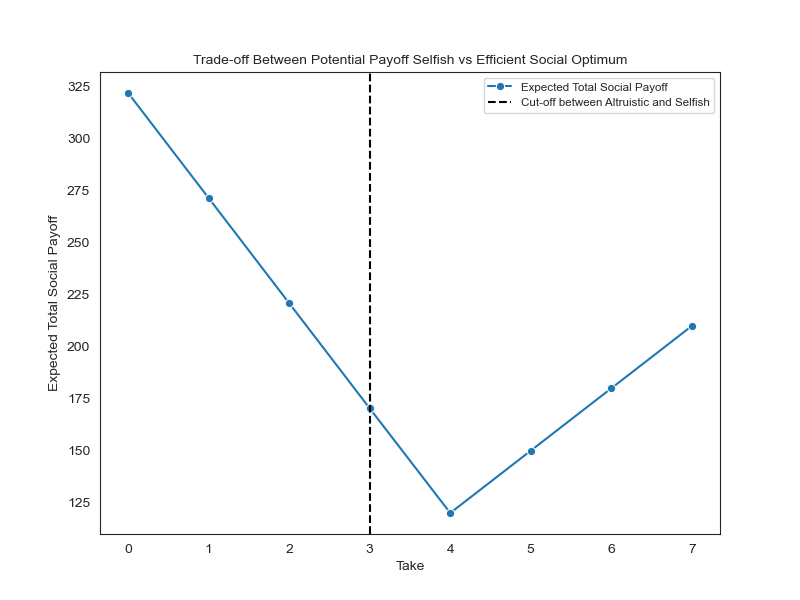
\includegraphics[width=0.8\linewidth]{../bld/graphs/0.Tradeoff3.png}
  \caption{Nash Equilibrium and Cooperative Equilibrium}\label{fig:tradeoff4}
\end{figure}

\noindent The red line in figure\ref{fig:tradeoff4} marks the cooperative equilibrium in the previous games. Notice how extracting less than 3 trees will improve society's expected payoff significantly. However, in the Anticipation game, there are 12 groups who experienced shock at the end of Round 5 while the other 12 did not experience any shock. The purpose of this Scarcity Game is precisely to test whether groups who previously have experienced scarcity subsequently extract more than their counterpart, due to the desire to secure payoff for oneself knowing that there are limited number of resources available. Hence, for groups with prior experience of scarcity, will not try to achieve social optimality as described in our Cooperative Equilibrium, while those who did not experience shock prior to Scarcity Game will extract less.
